\documentclass{beamer}
%\usepackage{beamerthemeBerkeley}
% Use either the one above or the one below
\usetheme{CambridgeUS}
%\usepackage{graphicx,color}
%\usepackage{lmodern}
%\usepackage{colortbl}

\usepackage{tikz}
%\usetikzlibrary{matrix,arrows,positioning}
\usepackage{algpseudocode}

\title{Datalog extensions}
\author{Simone de Oliveira Santos}
%\date{\today}

\begin{document}

\frame{\titlepage}

%\section[Outline]{}
%\frame{\tableofcontents}

\section[SociaLite]{SociaLite: Datalog extensions for efficient Social network analysis}
\subsection{Introduction}
\frame
{
	\frametitle{SociaLite: Datalog extensions for efficient Social network analysis}

	\textbf{Motivations}
	
	\begin{itemize}
		\item Rize of a large number of online social networks;
		\item Analysis are often built on top of fundamental \underline{graph algorithms};
		\item Need for a better computation model or query language to achieve the goal of letting consumers express queries on their personal social graphs;
		\item Datalog is a candidate for achieve this vision because of its high-level declarative semantics and support for recursion;		
	\end{itemize}
	
}

\frame
{
	\frametitle{SociaLite: Datalog extensions for efficient Social network analysis}

	\textbf{Motivations}
	
	\begin{itemize}
	\item However, the \underline{relational representation} in Datalog is \underline{not} a good match for graph analysis.
	\item The performance of Datalog is not competitive when compared with other languages (such as Java) for social network analysis; 
	\item General-purpose languages are more difficult to write analysis programs.
	\end{itemize}
	
	\textbf{Goal}: an extension of Datalog that delivers performance similar to that of highly optimized Java programs.
}

\frame
{
	\frametitle{Contributions}

	SociaLite allows concise expression of \underline{graph algorithms}, giving some degree of control over data layout and evaluation order.
	\begin{itemize}
	\item Tail-nested tables (new data representation)
	\item Recursive aggregate functions
	\item User-guide execution order
	\item Evaluation of SociaLite
	\end{itemize}
}


\frame
{
	\frametitle{Tail-Nested Tables}
	
	\begin{block}{Data as indices}
		Number data items sequentially and use the number as an index into an array, i.e., \textit{src:0..1000}.
	\end{block}

	\begin{block}{New data representantion to declare relations}
	EDGE(int src:0..10000, (int sink, int len))\footnote{tail-nested table}. \\
	PATH(int sink:0..10000, int dist).
	\end{block}
	
}

\frame
{
	\frametitle{Tail-Nested Tables}

	\begin{block}{}
	\centering
	EDGE(int src:0..10000, (int sink, int len))
	\end{block}
	
	\begin{figure}
		\centering
		\includegraphics[width=4cm]{tail_nested_table.png}
		\caption{Tail-nested table}
	\end{figure}
	
	Tail-nested table is a generalization of the adjacency list. The last column of a table may contain pointers to two-dimensional tables.
}

\frame
{
	\frametitle{Recursive Aggregate Functions}
	
	\begin{itemize}
		\item The extension must have the capability to eliminate unnecessary tuples.
	\end{itemize}

	\begin{block}{The shortest-paths algorithm}
		$PATH(t,d) :- EDGE(1,t,d).$ \\
		\hspace{1.8cm} $:- PATH(s,d_{1}), EDGE(s,t,d_{2}),$ \\
		\hspace{2.4cm} $d = d_{1}+d_{2}.$ \\
		$ MINPATH(t,\$ MIN(d)) :- PATH(t,d). $
	\end{block}
	
	\begin{itemize}
		\item Do not stop in the presence of cycles.
		\item Slow due to unnecessary computation of sub-optimal distances.
	\end{itemize}
}

\frame
{
	\frametitle{Recursive Aggregate Functions}
	
	\begin{itemize}
		\item Aggregate functions are expressed as an argument in a head predicate;
		\item They are recursive if the head predicate is used as a body predicate as well.
	\end{itemize}

	\begin{block}{The shortest-paths algorithm}
		EDGE(int \textit{src:0..10000}, (int \textit{sink}, int \textit{len})). \\
		PATH(int \textit{sink:0..10000}, int \textit{dist}). \\
		PATH($t,\underline{\$MIN(d)}$) :- EDGE($1,t,d$); \\
		\hspace{3cm} :- PATH(s,$d_{1}$), EDGE($s,t,d_{2}$), \\
		\hspace{3.5cm} $d = d_{1}+d_{2}$
	\end{block}
}

\frame
{
	\frametitle{Recursive Aggregate Functions}

	\begin{itemize}
		\item Recursive aggregate function improves the ability to express graph algorithms;
		\item Without them the program generates all the possible paths before finding the minimum, and does not terminate in the presence of cycles;
		\item With them the program specifies that only the minimum paths are of interest, thus eliminating cycles.
	\end{itemize}
}

\subsection{Operational Semantics}
\frame
{
	\frametitle{The operational semantics of SociaLite}

	\begin{itemize}
		\item All rules are repeatedly evaluated until convergence is achieved;
		\item Only one argument of a head predicate can be an aggregate function;
		\item The others are the qualifying parameters for the aggregate function.
	\end{itemize}
	
}

\frame
{
	\frametitle{Greatest Fixed-Point semantics}

	\begin{block}{}
		An operation is a \textbf{meet operation} if it is \textit{idempotent}, \textit{commutative} and \textit{associative}; \\
		A meet operation defines a semi-lattice; it induces a \textit{partial order} $\sqsubseteq$ over a domain, such that the result of the operation for any two elements is the \underline{greatest lower bound} of the elements with respect to $\sqsubseteq$.
	\end{block}
	
	\begin{enumerate}
		\item $R^{\ast} = h(R^{\ast})=(g\circ f)(R^{\ast})$
		\item $R \sqsubseteq R^{\ast}$ for all $R$ such that $R = h(R)$
	\end{enumerate}
	
}

\frame
{
	\frametitle{Semi-Naive Evaluation}
	
	\begin{itemize}
		\item It avoids redundant computation by joining only subgoals in the body of each rule with at least one new answer produced in the previous iteration.
		\item It can be extended to recursive aggregate functions if they are meet operations.	
	\end{itemize}
	
	Input: A SociaLite program $h = g\circ f$, where $g: R\rightarrow R$ applies an aggregation function to each set of qualifying parameters and $f : R \rightarrow R$ represent the rest of the rules.
}

\frame
{
	\frametitle{Examples}
	
	\begin{columns}
	\begin{column}{0.5\textwidth}
	\centering
	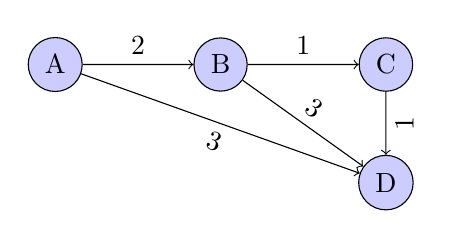
\begin{tikzpicture}
		[scale=.3,auto=midway]
		\node[circle,draw,fill=blue!20] (n1) at (2,10) {A};
		\node[circle,draw,fill=blue!20] (n2) at (9,10) {B};
		\node[circle,draw,fill=blue!20] (n3) at (16,10) {C};
		\node[circle,draw,fill=blue!20] (n4) at (16,5) {D};

		\draw[->] (n1) -- (n2) node[midway,sloped,above] {2};
		\draw[->] (n1) -- (n4) node[midway,sloped,below] {3};
		\draw[->] (n2) -- (n3) node[midway,sloped,above] {1};
		\draw[->] (n2) -- (n4) node[midway,sloped,above] {3};
		\draw[->] (n3) -- (n4) node[midway,sloped,below] {1};

	\end{tikzpicture}
	\end{column}
	
	\begin{column}{0.5\textwidth}
	
	\begin{figure}
		\centering
		\includegraphics[width=4cm]{tail_nested_table.png}
		\caption{Tail-nested table}
		\label{fig:tail_nested_table}
	\end{figure}
	
	\end{column}
	
	\end{columns}
}

\frame
{
	\frametitle{Examples}
	
	\begin{columns}
	
	\begin{column}{0.5 \textwidth}
	Method:
	\begin{algorithmic}
	\State $ R_{0} \gets \emptyset , \Delta_{0} \gets \emptyset $
	\State $i \gets 0$
	\Repeat
	\State $ i \gets 1+1 $
	\State $ R_{i} \gets g(f(\Delta_{i-1}) \cup R_{i-1}) $
	\State $ \Delta_{i} \gets R_{i}-R_{i-1}$
	\Until{$ \Delta_{i} \neq \emptyset $}
	
	\end{algorithmic}
	
	\end{column}
	
	\begin{column}{0.5\textwidth}
	
	\begin{block}{}
	$ f(R) = \{ < t,d > \mid 
	\newline
	EDGE(1,t,d) \vee 
	\newline 
	( <s,d_{1}> \in R \wedge EDGE(s,t,d_{2}) \wedge
	\newline
	 d = d_{1} + d_{2}) \} $
	\end{block}
	 
	 \begin{block}{}
	 $ g(R) = \{ <t,min_{<t,d_{1}> \in R}d_{1}> \mid
	 \newline
	 <t,d_{1}> \in R  \} $
	 \end{block}
	 
	\end{column}
	
	\end{columns}

}

\frame
{
	\frametitle{Examples}
	
	\begin{columns}	
	
	\begin{column}{0.5 \textwidth}
	\textit{Iteration 1:} \\
	Application of $f$ in $\Delta_{0}$ \\
	. \\
	$ f(R) = \{ < t,d > \mid 
	\newline
	EDGE(1,t,d) \vee 
	\newline 
	( <s,d_{1}> \in R \wedge EDGE(s,t,d_{2}) \wedge
	\newline
	 d = d_{1} + d_{2}) \} $
	
	. \newline
	
	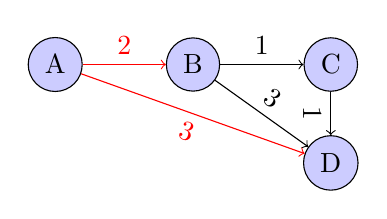
\begin{tikzpicture}
		[scale=.25,auto=midway]
		\node[circle,draw,fill=blue!20] (n1) at (2,10) {A};
		\node[circle,draw,fill=blue!20] (n2) at (9,10) {B};
		\node[circle,draw,fill=blue!20] (n3) at (16,10) {C};
		\node[circle,draw,fill=blue!20] (n4) at (16,5) {D};

		\draw[red][->] (n1) -- (n2) node[midway,sloped,above] {2};
		\draw[red][->] (n1) -- (n4) node[midway,sloped,below] {3};
		\draw[->] (n2) -- (n3) node[midway,sloped,above] {1};
		\draw[->] (n2) -- (n4) node[midway,sloped,above] {3};
		\draw[->] (n3) -- (n4) node[midway,sloped,below] {1};

	\end{tikzpicture}
	
	\end{column}
	
	\begin{column}{0.5\textwidth}

	\begin{figure}
		\centering
		\includegraphics[width=4cm]{tail_nested_table_1.png}
		\caption{Tail-nested table}
		\label{fig:tail_nested_table_1}
	\end{figure}	
	
	\centering
	\{PATH(B,2), PATH(D,3)\}
	
	\end{column}
	
	\end{columns}
}

\frame
{
	\frametitle{Examples}
	\begin{columns}	
	
	\begin{column}{0.5 \textwidth}
	Application of $G$ in $ \{ PATH(B,2), PATH(D,3) \}.
	\newline
	\newline
	g(R) = \{ <t,min_{<t,d_{1}> \in R}d_{1}> \mid
	\newline
	<t,d_{1}> \in R  \} $
	
	Result:
	$R_{1} = \{ PATH(B,2), PATH(D,3) \} $
		
	\end{column}
	
	\begin{column}{0.5\textwidth}
	Application of $\Delta$ \\
	$ \Delta_{i} \gets R_{i} - R_{i-1} $
	\\
	$ R_{0} = \emptyset$
	\\
	$ R_{1} = \{ PATH(B,2), PATH(D,3) \} $
	\\
	Result:
	$ \Delta_{1} = \{ PATH(B,2), PATH(D,3) \} $

	\end{column}
	
	\end{columns}
}

\frame
{
	\frametitle{Examples}
	\begin{columns}	
	
	\begin{column}{0.5 \textwidth}
	
	\textit{Iteration 2:} \\
	Application of $f$ in $\Delta_{1}$ \\
	$\Delta_{1} = \{PATH(B,2), PATH(D,3)\}$ \\
	. \\
	$ f(R) = \{ < t,d > \mid 
	\newline
	EDGE(1,t,d) \vee 
	\newline 
	( <s,d_{1}> \in R \wedge EDGE(s,t,d_{2}) \wedge
	\newline
	 d = d_{1} + d_{2}) \} $ \\
	. \\
	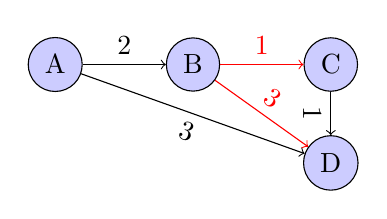
\begin{tikzpicture}
		[scale=.25,auto=midway]
		\node[circle,draw,fill=blue!20] (n1) at (2,10) {A};
		\node[circle,draw,fill=blue!20] (n2) at (9,10) {B};
		\node[circle,draw,fill=blue!20] (n3) at (16,10) {C};
		\node[circle,draw,fill=blue!20] (n4) at (16,5) {D};

		\draw[->] (n1) -- (n2) node[midway,sloped,above] {2};
		\draw[->] (n1) -- (n4) node[midway,sloped,below] {3};
		\draw[red][->] (n2) -- (n3) node[midway,sloped,above] {1};
		\draw[red][->] (n2) -- (n4) node[midway,sloped,above] {3};
		\draw[->] (n3) -- (n4) node[midway,sloped,below] {1};

	\end{tikzpicture}
	
	\end{column}
	
	\begin{column}{0.5\textwidth}

	\begin{figure}
		\centering
		\includegraphics[width=4cm]{tail_nested_table_2.png}
		\caption{Tail-nested table}
	\end{figure}	
	
	\centering
	\{PATH(B,2), PATH(D,3), PATH(C,3), PATH(D,5)\}
	
	\end{column}
	
	\end{columns}
}

\frame
{
	\frametitle{Examples}
	\begin{columns}	
	
	\begin{column}{0.5 \textwidth}
	
	Application of $G$ in $ \{ PATH(B,2), PATH(D,3), 
	\newline
	PATH(C,3), PATH(D,5) \}.
	\newline
	\newline
	g(R) = \{ <t,min_{<t,d_{1}> \in R}d_{1}> \mid
	\newline
	<t,d_{1}> \in R  \} $
	
	Result: \\
	$R_{2} = \{ PATH(B,2), PATH(D,3), 
	\newline
	PATH(C,3)\} $
	
	\end{column}
	
	\begin{column}{0.5\textwidth}
	
	Application of $\Delta_{2}$ \\
	$ \Delta_{2} \gets R_{2} - R_{1} $
	\\
	$ R_{1} = \{ PATH(B,2), PATH(D,3) \} $
	\\
	$ R_{2} = \{ PATH(B,2), PATH(D,3), 
	\newline
	PATH(C,3) \} $
	\\
	Result:\\
	$ \Delta_{2} = \{ PATH(C,3) \} $
	
	\end{column}
	
	\end{columns}	
}

\frame
{
	\frametitle{Examples}
	\begin{columns}	
	
	\begin{column}{0.5 \textwidth}
	
	\textit{Iteration 3:} \\
	Application of $f$ in $\Delta_{2}$ \\
	$\Delta_{2} = \{PATH(C,3)\}$ \\
	. \\
	$ f(R) = \{ < t,d > \mid 
	\newline
	EDGE(1,t,d) \vee 
	\newline 
	( <s,d_{1}> \in R \wedge EDGE(s,t,d_{2}) \wedge
	\newline
	 d = d_{1} + d_{2}) \} $ \\
	
	. \\
	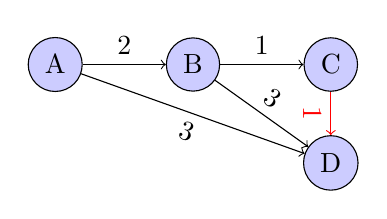
\begin{tikzpicture}
		[scale=.25,auto=midway]
		\node[circle,draw,fill=blue!20] (n1) at (2,10) {A};
		\node[circle,draw,fill=blue!20] (n2) at (9,10) {B};
		\node[circle,draw,fill=blue!20] (n3) at (16,10) {C};
		\node[circle,draw,fill=blue!20] (n4) at (16,5) {D};

		\draw[->] (n1) -- (n2) node[midway,sloped,above] {2};
		\draw[->] (n1) -- (n4) node[midway,sloped,below] {3};
		\draw[->] (n2) -- (n3) node[midway,sloped,above] {1};
		\draw[->] (n2) -- (n4) node[midway,sloped,above] {3};
		\draw[red][->] (n3) -- (n4) node[midway,sloped,below] {1};

	\end{tikzpicture}
	
	\end{column}
	
	\begin{column}{0.5\textwidth}

	\begin{figure}
		\centering
		\includegraphics[width=4cm]{tail_nested_table_3.png}
		\caption{Tail-nested table}
		\label{fig:tail_nested_table_3}
	\end{figure}	
	
	\centering
	\{PATH(B,2),PATH(D,3),PATH(D,4)\}
	
	\end{column}
	
	\end{columns}
}

\frame
{
	\frametitle{Examples}
	\begin{columns}	
	
	\begin{column}{0.5 \textwidth}
	Application of $G$ in $ \{ PATH(B,2), PATH(D,3), 
		\newline
		PATH(C,3), PATH(D,4) \}.
	\newline
	\newline
	g(R) = \{ <t,min_{<t,d_{1}> \in R}d_{1}> \mid
	\newline
	<t,d_{1}> \in R  \} $
	
	Result: \\
	$ R_{3} = \{ PATH(B,2), PATH(D,3), 
	\newline
	PATH(C,3)\} $
	
	\end{column}
	
	\begin{column}{0.5\textwidth}
	Application of $\Delta_{3}$ \\
	$ \Delta_{3} \gets R_{3} - R_{2} $
	\\
	$ R_{2} = \{ PATH(B,2), PATH(D,3), 
	\newline
	PATH(C,3) \} $
	\\
	$ R_{3} = \{ PATH(B,2), PATH(D,3), 
	\newline
	PATH(C,3) \} $
	\\
	Result:\\
	$ \Delta_{3} = \emptyset $
	\\
	Algorithm stops \\
	Return $R_{3}$
	
	\end{column}
	
	\end{columns}		



}

\subsection{Ordering}
\frame{
	\frametitle{Ordering}

	SociaLite lets users control the order in which the graphs are traversed. The programmer can declare that a column in a table is to be sorted (similar to SQL).\\
	\begin{center}
	$R(<type>f_{1},<type>f_{2,\dots})$ orderby[asc$\mid$desc],$\dots$
	\end{center}
	
	
	When a sorted column is included in a rule, it indicates to the compiler that the rows are to be evaluated in the order specified.


}

\frame{

	\begin{block}{User-Specified Funtions}
	Users can supply natively implemented functions and use them in SociaLite rules. A Java function $F$ with $n$ arguments can be invoked in SociaLite with \$$F(a_{1},\dots,a_{n})$, which can return one or more results.
	\end{block}
	
	\begin{block}{}
	SociaLite has pre-defined aggregate functions such as \$SUM, \$MIN, and \$MAX.
	\end{block}

	\begin{block}{}
	The SociaLite compiler accepts a SociaLite program, together with additional Java functions, and translates it into Java source code.
	\end{block}

}

\subsection{System overview}
\frame
{
	\frametitle{System overview}
	
	\begin{figure}
	\centering
	\includegraphics[width=10cm]{sociaLite_system.png}
	%\caption{Our own test of downsampling}
	\label{fig:sociaLite_system}
	\end{figure}
}


\section[Distributed SociaLite]{Distributed SociaLite: A Datalog-Based Language for Large-Scale Graph Analysis}
\frame
{
	\frametitle{Extension of SociaLite}
	\begin{block}{}
		Distributed SociaLite: A Datalog-Based Language for Large-Scale Graph Analysis
	\end{block}
	
	With distributed SociaLite, \underline{programmers simply annotate how data are to be distributed}, then the necessary communication is automatically inferred to generate parallel code for cluster of multi-core machines.
	
%	\begin{block}{Process large-scale distributed systems}
%		\begin{itemize}
%			\item Map-Reduce cannot be easily express social network analyses;
%			\item Pregel is one of the most well-known languages in response to these issues.
%		\end{itemize}
%	\end{block}

}

\frame
{
	\frametitle{Extension of SociaLite}
	\begin{figure}
		\centering
		\includegraphics[width=8cm]{comparison.png}
		\caption{Comparison Datalog extension}
	\end{figure}
	
}

\section[The WebdamLog System]{The WebdamLog System: Managing Distributed Knowledge on the Web}
\frame
{
	\frametitle{The WebdamLog System}
	
	Motivations
	\begin{itemize}
		\item The need for a unified approach for the management of distributed content;
		\item Personal information management;
		\item A declarative language to facilitate the adoption of our platform by non-technical users.
	\end{itemize}
	Goal: A declarative high-level language in the style of Datalog, to support the distribution of both data and knowledge over a network of heterogeneous peers.
}

\frame
{
	\frametitle{Overview}
	
	\textbf{WebdamLog} is a datalog-style language that emphasizes cooperation between distributed autonomous peers communication in an asynchronous manner, and supports
	\begin{itemize}
		\item updates
		\item distribution
		\item negation
		\item delegation
	\end{itemize}	
}


\frame
{
	\frametitle{Example}
	
	Making a photo album of Alice and Bob using photos of closer friends. \\
	\textbf{Tasks:}
	\begin{enumerate}
		\item identify friends using social networks;
		\item find out where they keep their photos and how access them; 
		\item select photos with both Alice and Bob;
		\item ask a friend to verify if the photos are appropriate;
		\item exclude someone, if necessary, from the set of source.
	\end{enumerate}

	
}

\frame
{
	\frametitle{Example}
	
	Making a photo album of Alice and Bob using photos of closer friends. \\
	\textbf{Tasks:}
	\begin{enumerate}
		\item identify friends using social networks;
		\item 
		\item 
		\item 
		\item 
	\end{enumerate}

	\begin{block}{[rule at sue]}
		source@sue(\$name) :- friends@aliceFB(\$name) \\
		source@sue(\$name) :- friends@bobFB(\$name) \\
	\end{block}

	This rule computes the union of Alice's and Bob's Facebook contacts in relation \textit{source} on Sue's peer.
	
}

\frame
{
	\frametitle{Example}
	
	Making a photo album of Alice and Bob using photos of closer friends. \\
	\textbf{Tasks:}
	\begin{enumerate}
		\item 
		\item find out where they keep their photos and how access them; 
		\item select photos with both Alice and Bob;
		\item 
		\item 
	\end{enumerate}

	\begin{block}{[rule at sue]}
		album@sue(\$photo,\$name) :- source@sue(\$name), \\
		\hspace{2.5cm} photoLocation@\$name(\$peer), photos@\$peer(\$photo), \\
		\hspace{2.5cm} features@\$peer(\$photo,alice), features@\$peer(\$photo,bob) \\
	\end{block}

	This rule delegates steps (2) and (3) to the peers corresponding to the friends of Alice and Bob.
	
}

\frame
{
	\frametitle{Example}
	
	Making a photo album of Alice and Bob using photos of closer friends. \\
	\textbf{Tasks:}
	\begin{enumerate}
		\item 
		\item  
		\item 
		\item ask a friend to verify if the photos are appropriate;
		\item 
	\end{enumerate}

	\begin{block}{[rule at dan]}
		album@sue(\$photo,dan) :- photoLocation@dan(\$peer), \\
		\hspace{2.5cm} photos@\$peer(\$photo), features@\$peer(\$photo,alice) \\
		\hspace{2.5cm} features@\$peer(\$photo,bob) \\
	\end{block}

	Dan is a friend, then Sue's peer will delegate this rule to Dan's peer.
	
}

\frame
{
	\frametitle{Example}
	
	Making a photo album of Alice and Bob using photos of closer friends. \\
	\textbf{Tasks:}
	\begin{enumerate}
		\item 
		\item  
		\item 
		\item 
		\item exclude someone, if necessary, from the set of source.
	\end{enumerate}

	\begin{block}{[rule at sue]}
		source@sue(\$name) :- friends@aliceFB(\$name), not blocked@sue(\$name) \\
		source@sue(\$name) :- friends@bobFB(\$name), not blocked@sue(\$name) \\
	\end{block}

	By inserting/removing facts in \textit{blocked@sue}, Sue controls who can participate.
	
}

\subsection{Webdamlog Model}
\frame
{
	\frametitle{Webdamlog Model}
	
	Assuming the existence of a countable set of data values (set of relation names and set of peer names) and a countable set of variables. \\
	\begin{block}{\textbf{Relation} is an expression \textit{$m@p$} where:}
	\begin{itemize}
		\item \textit{m} is a relation name
		\item \textit{p} is a peer name
	\end{itemize}
	\end{block}

	\begin{block}{\textbf{Schema} is an expression \textit{$(\pi ,E,I,\sigma )$} where:}
	\begin{itemize}
		\item $\pi$ is a possibly infinite set of peer names
		\item $E$ is a set of extensional relations of the form $m@p$ for $ p \in \pi $
		\item $I$ is a set of intensional relations of the form $m@p$ for $ p \in \pi $
		\item $\sigma$, the sorting function, specifies for each relation $m@p$, an integer $\sigma(m@p)$ that is its sort (arity).
	\end{itemize}
	\end{block}	
		
}

\frame
{
	\frametitle{Webdamlog Model}
	
	\begin{block}{\textbf{Fact} is an expression $m@p(a_{1} \dots a_{n})$ where:}
	\begin{itemize}
		\item $n = \sigma(m@p)$
		\item $a_{1} \dots a_{n}$ are data values
	\end{itemize}
	An example of fact is: $picture@myalbum(1771.jpg, "Paris", 11/11/2011)$
	\end{block}	

	\begin{block}{\textbf{Rule} is an expression of the form:}
	[at $p$] $ \$R@\$P(\$U) :- (\neg) \$R_{1}@\$P_{1}(\$U_{1}), \dots , (\neg) \$R_{n}@\$P_{n}(\$U_{n}) $, where:
	\begin{itemize}
		\item $\$R, \$R_{i}$ are relation terms
		\item $\$P, \$P_{i}$ are peer terms
		\item $\$U, \$U_{i}$ are tuples of terms
	\end{itemize}
	\end{block}

}

\frame
{
	\frametitle{Webdamlog Model}
	
	At a particular point in time a peer \textit{p} has:
	\begin{itemize}
		\item a \textit{state} consisting of some facts
		\item some rules specified locally
		\item possibly some rules that have been delegated by other peer
	\end{itemize}

	Peers evolve by:
	\begin{itemize}
		\item updating their base of facts
		\item sending facts to other peers
		\item updating their delegations to other peers
	\end{itemize}

}

\frame
{
	\frametitle{Webdamlog Model}
	
	\begin{itemize}
		\item A rule is \textit{deductive} if the head relation is intensional. Otherwise, it is \textit{active}.
		\item A rule in a peer \textit{p} is \textit{local} if all $P_{i}$ in all body relations are from \textit{p}.
		\item A rule is \textit{fully local} if the head relation is also from \textit{p}.
	\end{itemize}
	
	A local computation happens at a particular peer. The peer performs the following:
	\begin{itemize}
		\item Some local deduction of intensional facts
		\item The derivation of extensional facts that either define its next state or are sent as messages
		\item The delegation of rules to other peers.
	\end{itemize}

}

\frame
{
	\frametitle{Webdamlog Model}

	Classes or rules:
	\begin{itemize}
		\item \textbf{Local deduction} Fully local deductive rules are used to derive intensional fats locally.
		\item \textbf{Update} Local active rules are used for sending messages, facts, that modify the databases of the others peers that receive them.
		\item \textbf{View delegation} Provide some form of view materialization. For instance, a rule result in providing at \textit{q} a view for some data from \textit{p}.
		\item \textbf{General delegation} The remaining rules allow a peer to install arbitrary rule at other peers.
	\end{itemize}

}

\frame
{
	\frametitle{Webdamlog Model}

	Convergence of WebdamLog
	\begin{itemize}
		\item Positive WebdamLog
		\item Strongly-stratified Webdamlog
	\end{itemize}





}

\frame
{
	\frametitle{The WebdamLog system}
	
	Extension of a existing datalog engine.
	\begin{itemize}
		\item \textbf{IRIS}, implemented in Java and supports the main strategies for efficient evaluation of standard local datalog
		\item \textbf{Bud}, implemented in Ruby scripting language, and provide mechanisms for asynchronous communication between peers. (the chosen)
	\end{itemize}

}

\end{document}
